\documentclass[MasterThesisMain.tex]{subfiles}
\begin{document}
	\chapter{Experimental method}\label{experimentalmethod}
	
In this chapter a general outline of polymer classification will be outlined with the addition of a description	of the polymers used in the solvent vapour annealing experiments. The spectrometer setup will be introduced and the necessary information related to how the spectrometer measures the reflectance of the thin films and the experimental measurement protocol. The reflectance data fitting will be explained and the chapter will close with a brief description of the mass flow meters controlling the annealing and the solvent vapour annealing process. 
	
\section{Polymers}
Polymers are long chains of molecular units called mers, linked together by covalent bonds. Polymers are both found in biological system and synthesised by chemists. Polymers are described by their properties such as its chemistry, stereochemistry, architecture and what phase it is in \cite{jones2002soft}. A polymers chemistry is what the polymer is built of and with different structures, the polymers display different properties. Homopolymers are polymers built of one type of mer, where block copolymers are built up of two types of mers, an A and B. The different properties of the polymer is also dependant on how the repeating molecular units are bonded together, this is called the polymers stereochemistry, for example a block copolymer can be structured as a long chain of the A polymers bonded to a long chain of the B polymer. Polymers can be polar and non-polar due to the valence electron preferring one element from another. The polymers architecture describes the general structure of the polymer, which can be linear, branched or cross-linked. Linear polymers are long chains of monomers with bonds that are rigid to a certain degree, and cannot rotate freely, and are normally strong structures. Branched polymers are long chains with side chains attached to the main chain. Theses side chains can be comprised of monomers and reactive groups. Branched polymers are normally more softer and less crystalline that linear polymers. Cross-linked polymers are two or more side chains joined together forming a loose two dimensional network. Cross-linked polymers are more rigid and burn rather than melt when heated. 

The architecture of a polymer can also be expressed with the degree of polymerisation, $N$, which characterises the average number of mers units in the chain. It is defined as:

\begin{equation}
N = \frac{\bar{M}_n}{\bar{m}},
\end{equation}
where $\bar{M}_n$ is the number average molecular weight and $\bar{m}$ is the mer molecular weight. The polymerisation of a block co polymer is the sum of the individual block polymerisation, $N = N_A + N_B$. The number average molecular weight is defined as:
\begin{equation}
\bar{M}_n = \frac{\sum N_iM_i}{\sum N_i} = \sum x_iM_i,
\end{equation}      
where $x_i = \frac{N_i}{\sum N_i}$ is the fraction of the number of chains with a corresponding size range $i$ and $M_i$ is mean molecular weight in the size range $i$. The weight average molecular weight for a polymer is defined as:
\begin{equation}
\bar{M}_w=\frac{\sum N_iM_i^2}{\sum N_iM_i},
\end{equation}
where $N_i$ is the number of polymers with weight $M_i$. There is a dispersion of different polymer sizes in a solution, this dispersion is called the polydispersion index of the polymer and is expressed as:

\begin{equation}
PDI = \frac{\bar{M}_w}{\bar{M}_n},
\end{equation} 

where $\bar{M}_w$ is the weight average molecular weight and $\bar{M}_n$ is the number average molecular weight \cite{strobl2007physics}.

The block co polymers can be further described by the volume fraction $f$ that the different blocks take up and be the Flory-Huggins interaction parameter $\chi$ which describes the degree of incompatibility between the two polymers. The volume fraction of A and B blocks are respectively:

\begin{equation}
f_A = \frac{V_A}{V_{total}} \quad f_B=\frac{V_B}{V_{total}}.
\end{equation}

The Flory-Huggins interaction parameter is determine experimentally and expressed as:

\begin{equation}
\chi(T) = \frac{\chi_H}{T} + \chi_S,
\end{equation} 
where $\chi_H$ is of due to enthalpy and $\chi_S$ is due to entropy. Chemically dissimilar polymers tend to display a larger $\chi$ value than chemically similar,\cite{BCPthermo}\cite{FHpolymer}.

The polymers can also be in a physical state at a given temperature. The chemistry and architecture defines at what temperature the polymer undergoes a phase transition. A polymer can melt and transition into a liquid, which is often very viscous with viscoelastic properties. A polymer has trouble crystallising, polymers are most often in a glassy phase below the glass transition temperature $T_g$, a glassy phase is described as amorphous since the structure resembles both a liquid and a solid. A polymer can crystallise but the crystallisation is not complete because of the polymers architecture. This is called a semi-crystalline state where the polymer has regions behaving liquid like and glass like. And lastly a polymer can be in a liquid crystalline state which involves rigid polymers forming layers \cite{petty2008molecular}. 

Micro-phase segregation of block copolymers is seen and understood as a thermodynamic process, in which the blocks of the polymer have a thermodynamic incompatibly described by Flory-Huggins interaction parameter $\chi_{AB}$, which creates a nanoscale structure. The covalent bond between block A and block B prevent macro-phase separation, and micro-phase segregation occurs.  This leads to the application of block copolymers as self-assembling structures that can be created on a surface and used for nanoscale devices. The applications span across a multitude of disciplines such as separation membranes, nanofludics, photonics and biological scaffolds. The block copolymers self-assembling properties depend on the mobility of the polymer chains before structional reorganisation can proceed. This is normally done by thermal treatements above the polymers glass transition temperature $T_g$, but with high molar mass system long annealing times are need \cite{SVABCP}.

\section{Polymers used in Solvent Vapour Annealing}
In this section the homopolymers Polystyrene and Polyisoprene and the block copolymer Polystyrene-b-Polyisoprene properties will be presented.  

\subsection{Homopolymer Chemistry}
\newcommand\setpolymerdelim[2]{\def\delimleft{#1}\def\delimright{#2}}
\def\makebraces[#1,#2]#3#4#5{%
\edef\delimhalfdim{\the\dimexpr(#1+#2)/2}%
\edef\delimvshift{\the\dimexpr(#1-#2)/2}%
\chemmove{%
\node[at=(#4),yshift=(\delimvshift)]
{$\left\delimleft\vrule height\delimhalfdim depth\delimhalfdim
width0pt\right.$};%
\node[at=(#5),yshift=(\delimvshift)]
{$\left.\vrule height\delimhalfdim depth\delimhalfdim
width0pt\right\delimright_{\rlap{$\scriptstyle#3$}}$};}}


\setpolymerdelim[]
Polystyrene \ce{(C8H8)_N}:
\chemfig{-[@{left,0.3},1.5]C(-[:90]*6(=-=-=-))(-[6]H)-C(-[2]H)(-[6]H)-[@{right,0.8}]}
\makebraces[90pt,30pt]{N}{left}{right}
\bigskip


\setpolymerdelim[]
Polyisoprene \ce{(C5H8)_N}:
\chemfig{-[@{left,0.3},1.5]CH_2-CH=C(-[6]CH_3)-CH_2-[@{right,0.8}]}
\makebraces[10pt,15pt]{N}{left}{right}

%\setpolymerdelim[]
%Poly(methyl methacrylate) \ce{(C5O2H8)_n}:
%\chemfig{-[@{left,0.3},1.5]CH_2-CH=C(-[6]CH_3)-CH_2-[@{right,0.8}]}
%\makebraces[10pt,15pt]{n}{left}{right}

\section{Polymer Considerations}
Before commencing solvent vapour annealing some consideration is need into what polymers, what solvent and what substrate should be used. Polystyrene has been chosen as block A of the block copolymer and Polyisoprene chosen as block B. Polystyrene is in the glassy phase at room temperature, where polyisoprene is in a rubbery phase at room temperature. The morphology of the block can shed a light on how the vapour could interact with the blocks during solvent vapour annealing. The molar mass, polymerisation of both block, polydispersion index and the interaction parameter between the two block is helpful to understand what might happen during the solvent vapour annealing process. High molar mass systems are strongly segregated and take longer to come into equilibrium than a lower molar mass system. Interaction between the solvent and the polymers will also give insight into how the morphology could evolve during the solvent vapour annealing.

\subsection{Relevant values}

\begin{tabular}{ |p{3cm}||p{3cm}|p{3cm}|p{3cm}|  }
 \hline
 \multicolumn{4}{|c|}{Polymer Values} \\
 \hline
    & Polystyrene & Polyisoprene & PS-b-PI\\
 \hline
 $T_g$& $\SI{379}{\kelvin}$   & $\SI{204}{\kelvin}$  &   \\
 $N$&  &  &  \\
 $N_A$&  &  &  \\
 $N_B$&  &  &  \\
 $f_A$&  &  &  \\
 $f_B$&  &  &  \\
 $\bar{M}_n$&  &  &  \\
 $\bar{M}_w$&  &  &  \\
 $PDI$&  &  &  \\
 $\chi$&  &  &  \\
 $n$& $1.60$ & $1.51$ &\\
 \hline
\end{tabular}

\subsection{List of polymers used in experiments}

\begin{tabular}{ |p{3cm}||p{2cm}|p{2cm}|p{2cm}|p{2cm}|p{2cm}|  }
 \hline
 \multicolumn{6}{|c|}{Polymer used in experiments} \\
 \hline
 Experiment & Polymer & ID & Spincoat Thickness & Static Measurement Thickness & Static Refractive Index\\
 \hline
 Light Source Fluctuation & Polystyrene & 349 & $\approx\SI{200}{\nano\meter}$ & $\SI{280.4}{\nano\meter}$ & $1.5944$  \\
 SVA Ambient Study & Topsil Blank & N/A & SiOx-layer$\SI{2}{\nano\meter}$ & N/A & N/A  \\
 Polystyrene Swelling & PS  & 348  & $\approx\SI{200}{\nano\meter}$ & $\SI{275.5}{\nano\meter}$ & $1.5975$  \\
 Polyisoprene Swelling & PI  & 353 & $\approx\SI{200}{\nano\meter}$ & $\SI{301}{\nano\meter}$ & $1.4594$  \\
 Polystyrene-b-Polyiosprene & PS-b-PI & 370 & $\approx\SI{100}{\nano\meter}$ & $\SI{97.3}{\nano\meter}$ & $1.5659$  \\
 \hline
\end{tabular}

\section{Spin Coating thin films}
Spin coating is the deposition method used to fabricate the thin films used in this thesis. This is a wet method where a polymer is dissolved in a solution then deposited onto the semiconductor wafer, silicon wafer. The silicon wafer is rotated at a fixed low rpm to spread the polymer solution across the wafer. The rpm is increased spinning off the excess solution and will evaporate leaving a thin film with uniform thickness. This method is predicted by the following expression:

\begin{equation}
d = \left(\frac{\eta}{4\pi\rho\omega^2}\right)^{\frac{1}{2}} t^{-\frac{1}{2}},
\end{equation}  
where d is the predicted thickness, $\eta$ the viscosity coefficient of the polymer solution, $\rho$ solution density, $\omega$ angular velocity of the spinning and $t$ is the spinning time \cite{petty2008molecular}. The spin coated block copolymers show defect-rich morphologies due to fast evaporation of the solvent and the polymers being in a thermal non-equilibrium \cite{PosseltBCP}.

\section{Spectrometer Setup}
The experimental setup is comprised of a NanoCalc XR and a Halogen light source(HL-2000-FHSA) seen in figure \ref{fig:speclight}, which can produce wavelengths of \SI{360}{\nano\meter} to \SI{2400}{\nano\meter}. When the samples are being measured they are either placed on the ocean optics single point stage seen in figure \ref{fig:Singlestage} or in the solvent vapour annealing (SVA) experimental chamber seen in figure \ref{fig:SVAchamber} made by the IMFUFA(Indsatsområdet for Studiet af Matematik og Fysik samt deres Funktioner i Undervisning, Forskning og Anvendelser) workshop for small angle x-ray scattering (SAXS) and and grazing incidence small angle x-ray scattering(GISAXS) experiments. The NanoCalc is comprised of a spectrometer and an internal light source as seen in the figure \ref{fig:nanocalcsetup}, which can produce wavelengths of \SI{250}{\nano\meter} to \SI{1050}{\nano\meter} and measure thicknesses of \SI{10}{\nano\meter} to \SI{100}{\micro\meter}. The NanoCalc XR is connected to a computer where the NanoCalc software is installed and operated. For the experiments the halogen light source is used since it has a larger output power then the internal light source of the NanoCalc XR. The larger intensity output is need when performing experiments in the SVA experimental chamber. The lid of the SVA experimental chamber holds the optical fiber and light passes through a sapphire lens before entering the chamber and illuminate the thin film. The sapphire lens is need to focus the light upon the thin film due to the distance from the optical fiber to the sample is greater than the single point stage. Throughout this thesis "with optics" will be used when referring to measurement taken using the SVA experimental chamber since the light passes through the sapphire lens. "Without optics" refers taking measurements using the single point stage.  

For experiments done in this thesis white light is produced in the light source(HL-2000-FHSA), which travels through optical fiber and strikes that sample. The reflected light travels back through the optical fiber and the intensity across every wavelength of the white light is collected in the spectrometer and is sent to software created by in house and saved to a file and analysed in MATLAB\textsuperscript{\textregistered}.  
	
	\begin{figure}[ht] 
	  \begin{minipage}[b]{0.5\linewidth}
	    \centering
	    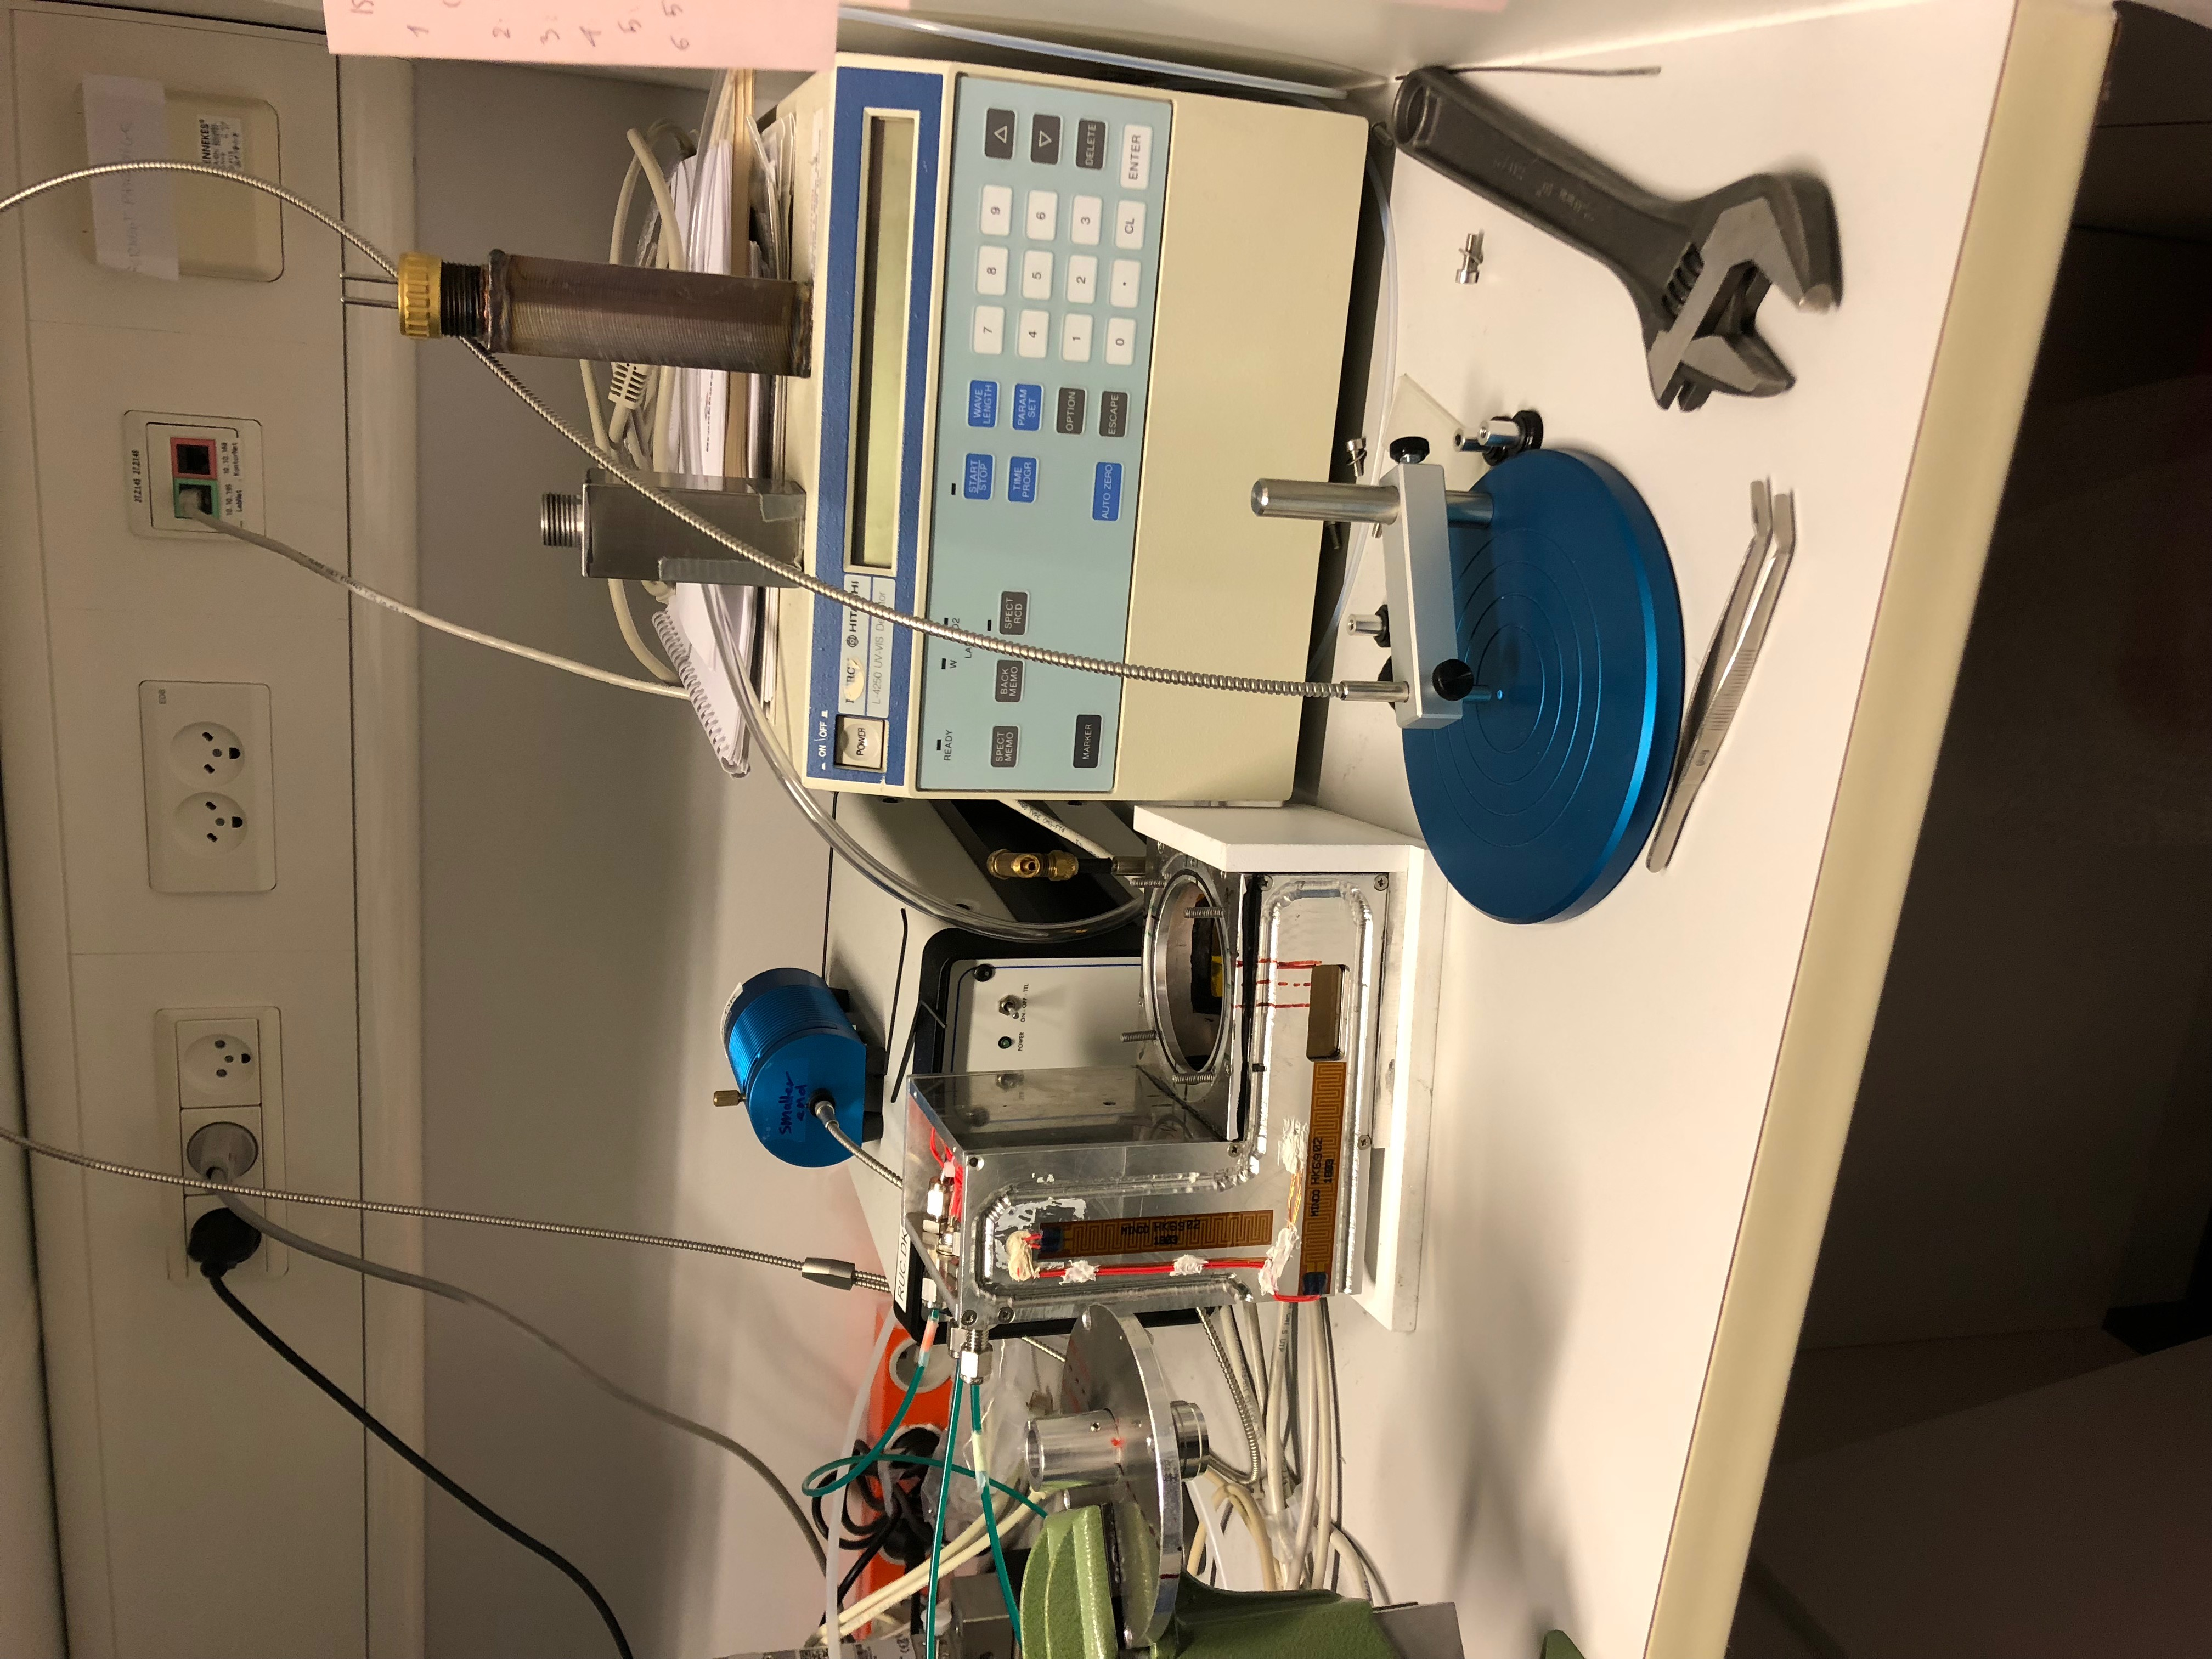
\includegraphics[width=.9\linewidth,angle=-90]{setup1.JPG} 
	    \caption{SVA experiment area}
	    \label{fig:exparea}  
	    \vspace{4ex}
	  \end{minipage}%%
	  \begin{minipage}[b]{0.5\linewidth}
	    \centering
	    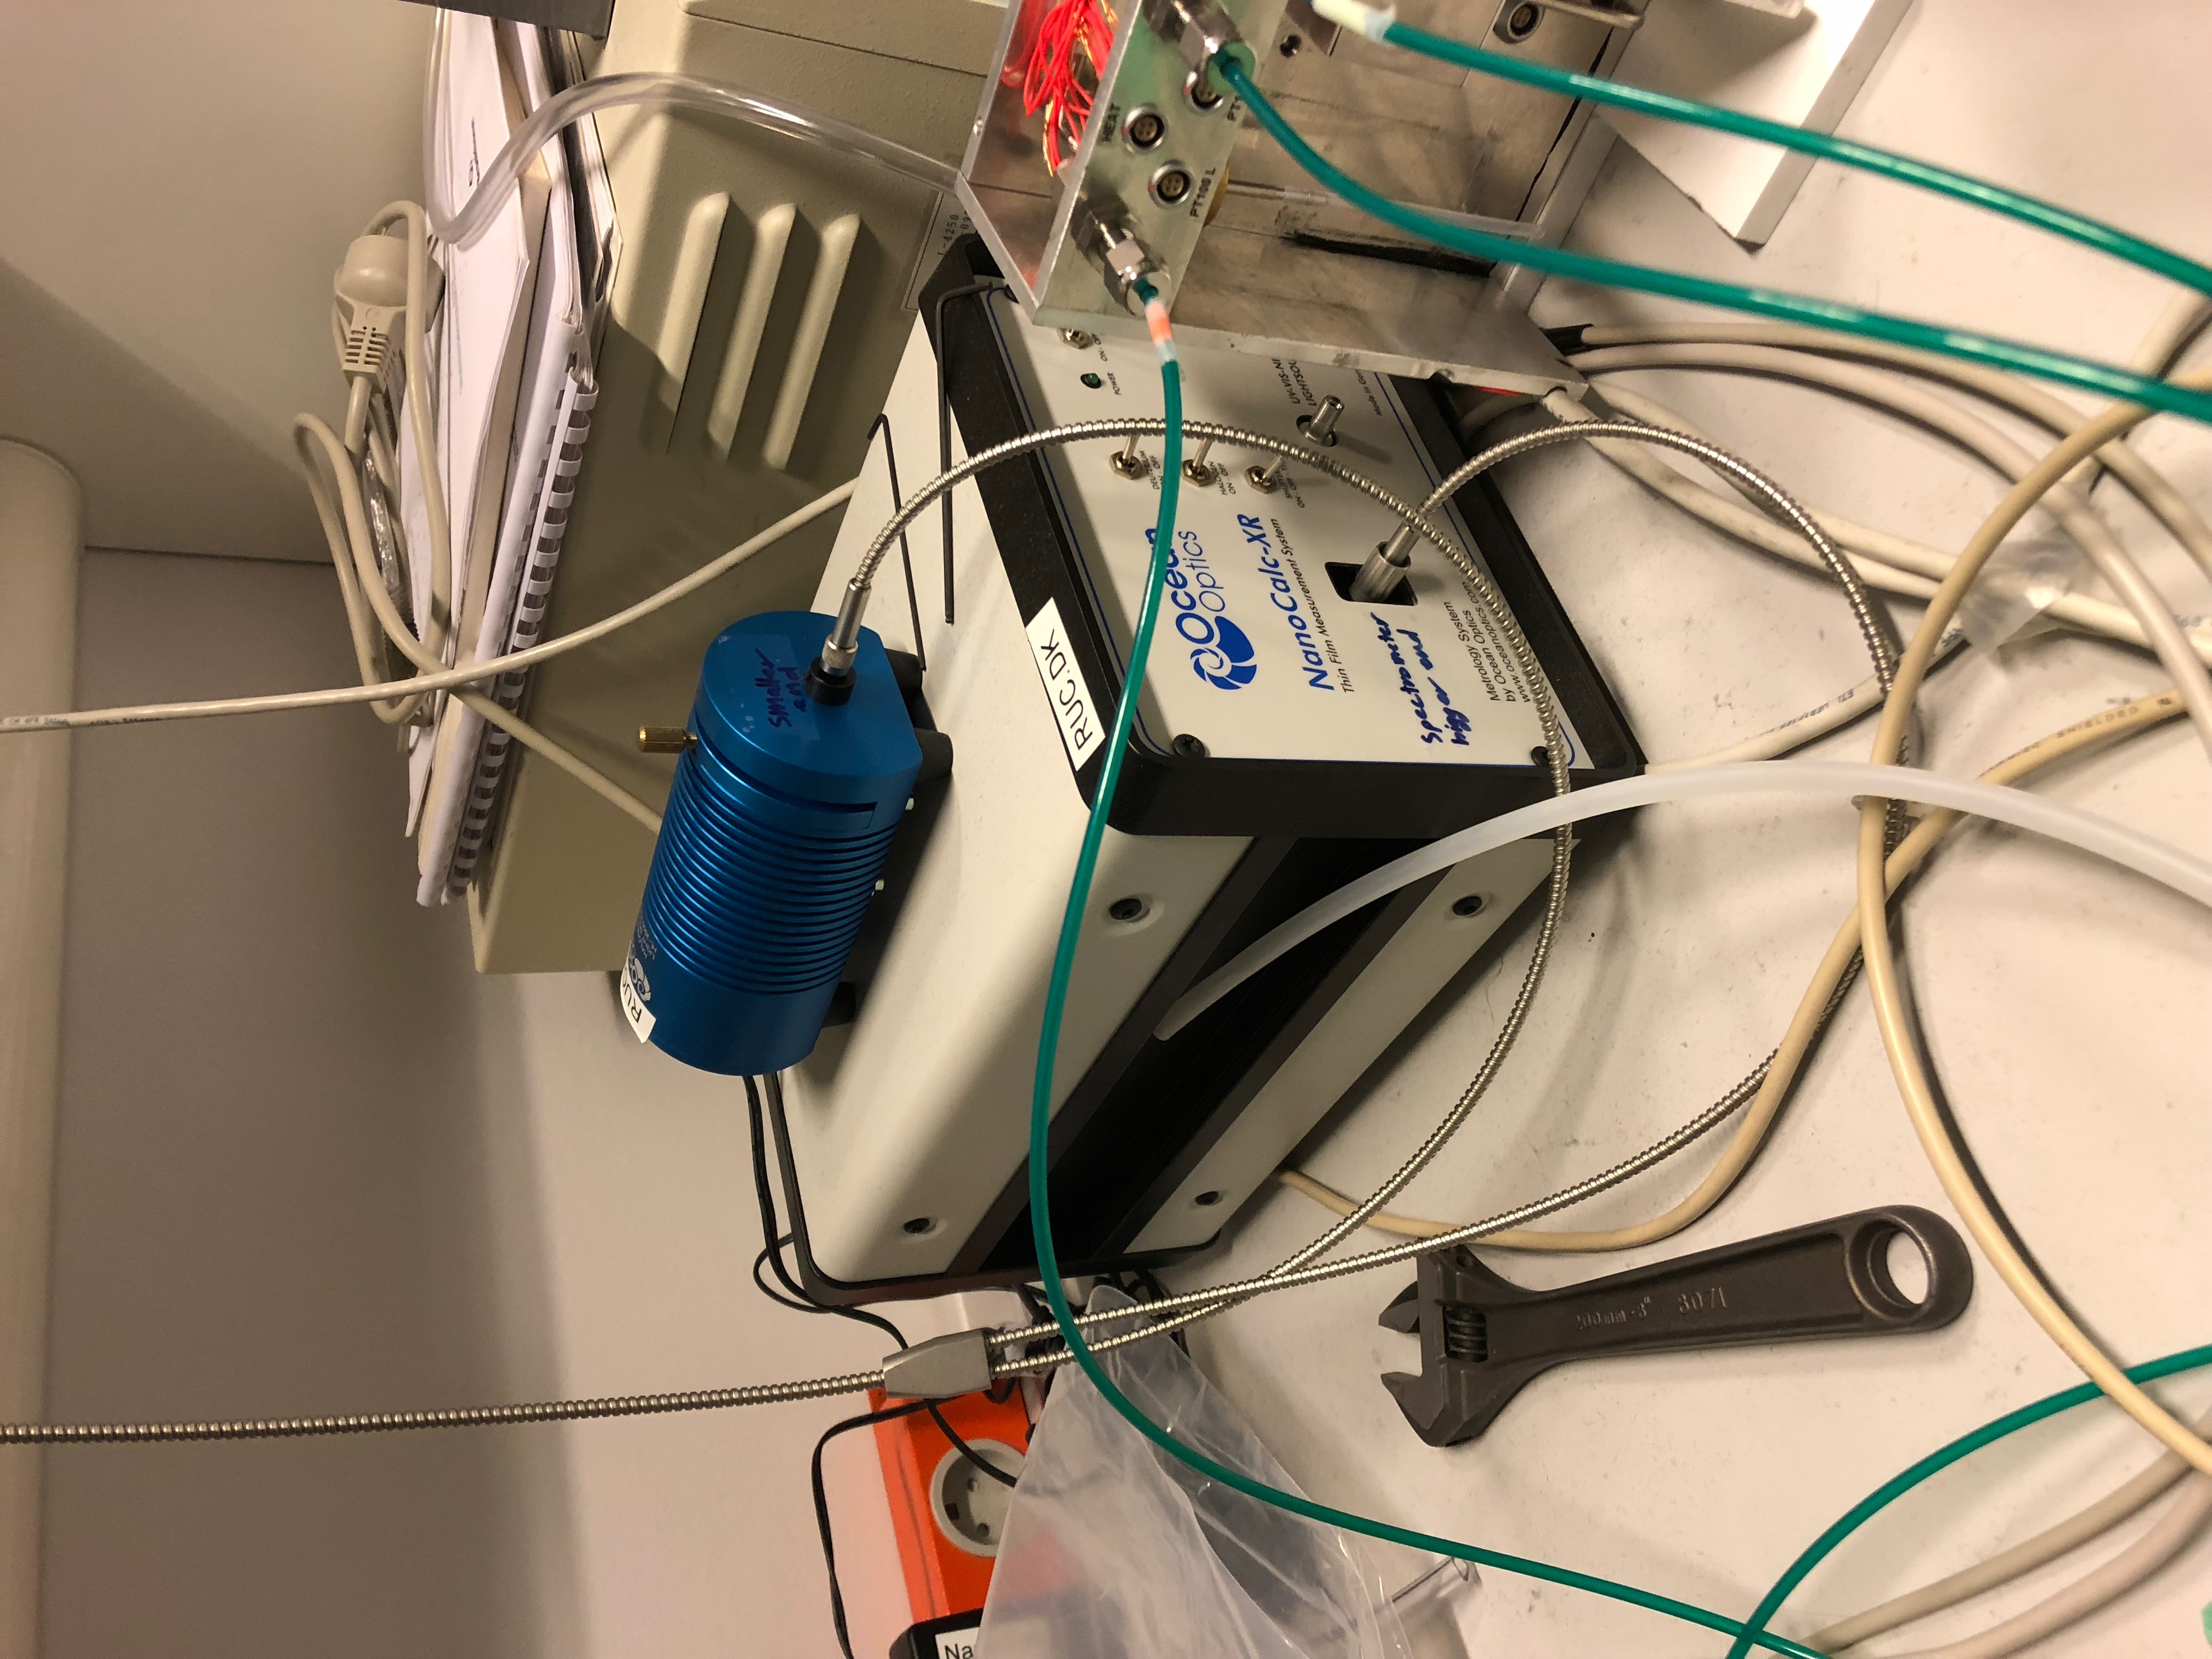
\includegraphics[width=.9\linewidth,angle=-90]{setup2.JPG} 
	    \caption{NanoCalc XR and a Halogen light source(HL-2000-FHSA)}
	    \label{fig:speclight} 
	    \vspace{4ex}
	  \end{minipage} 
	  \begin{minipage}[b]{0.5\linewidth}
	    \centering
	    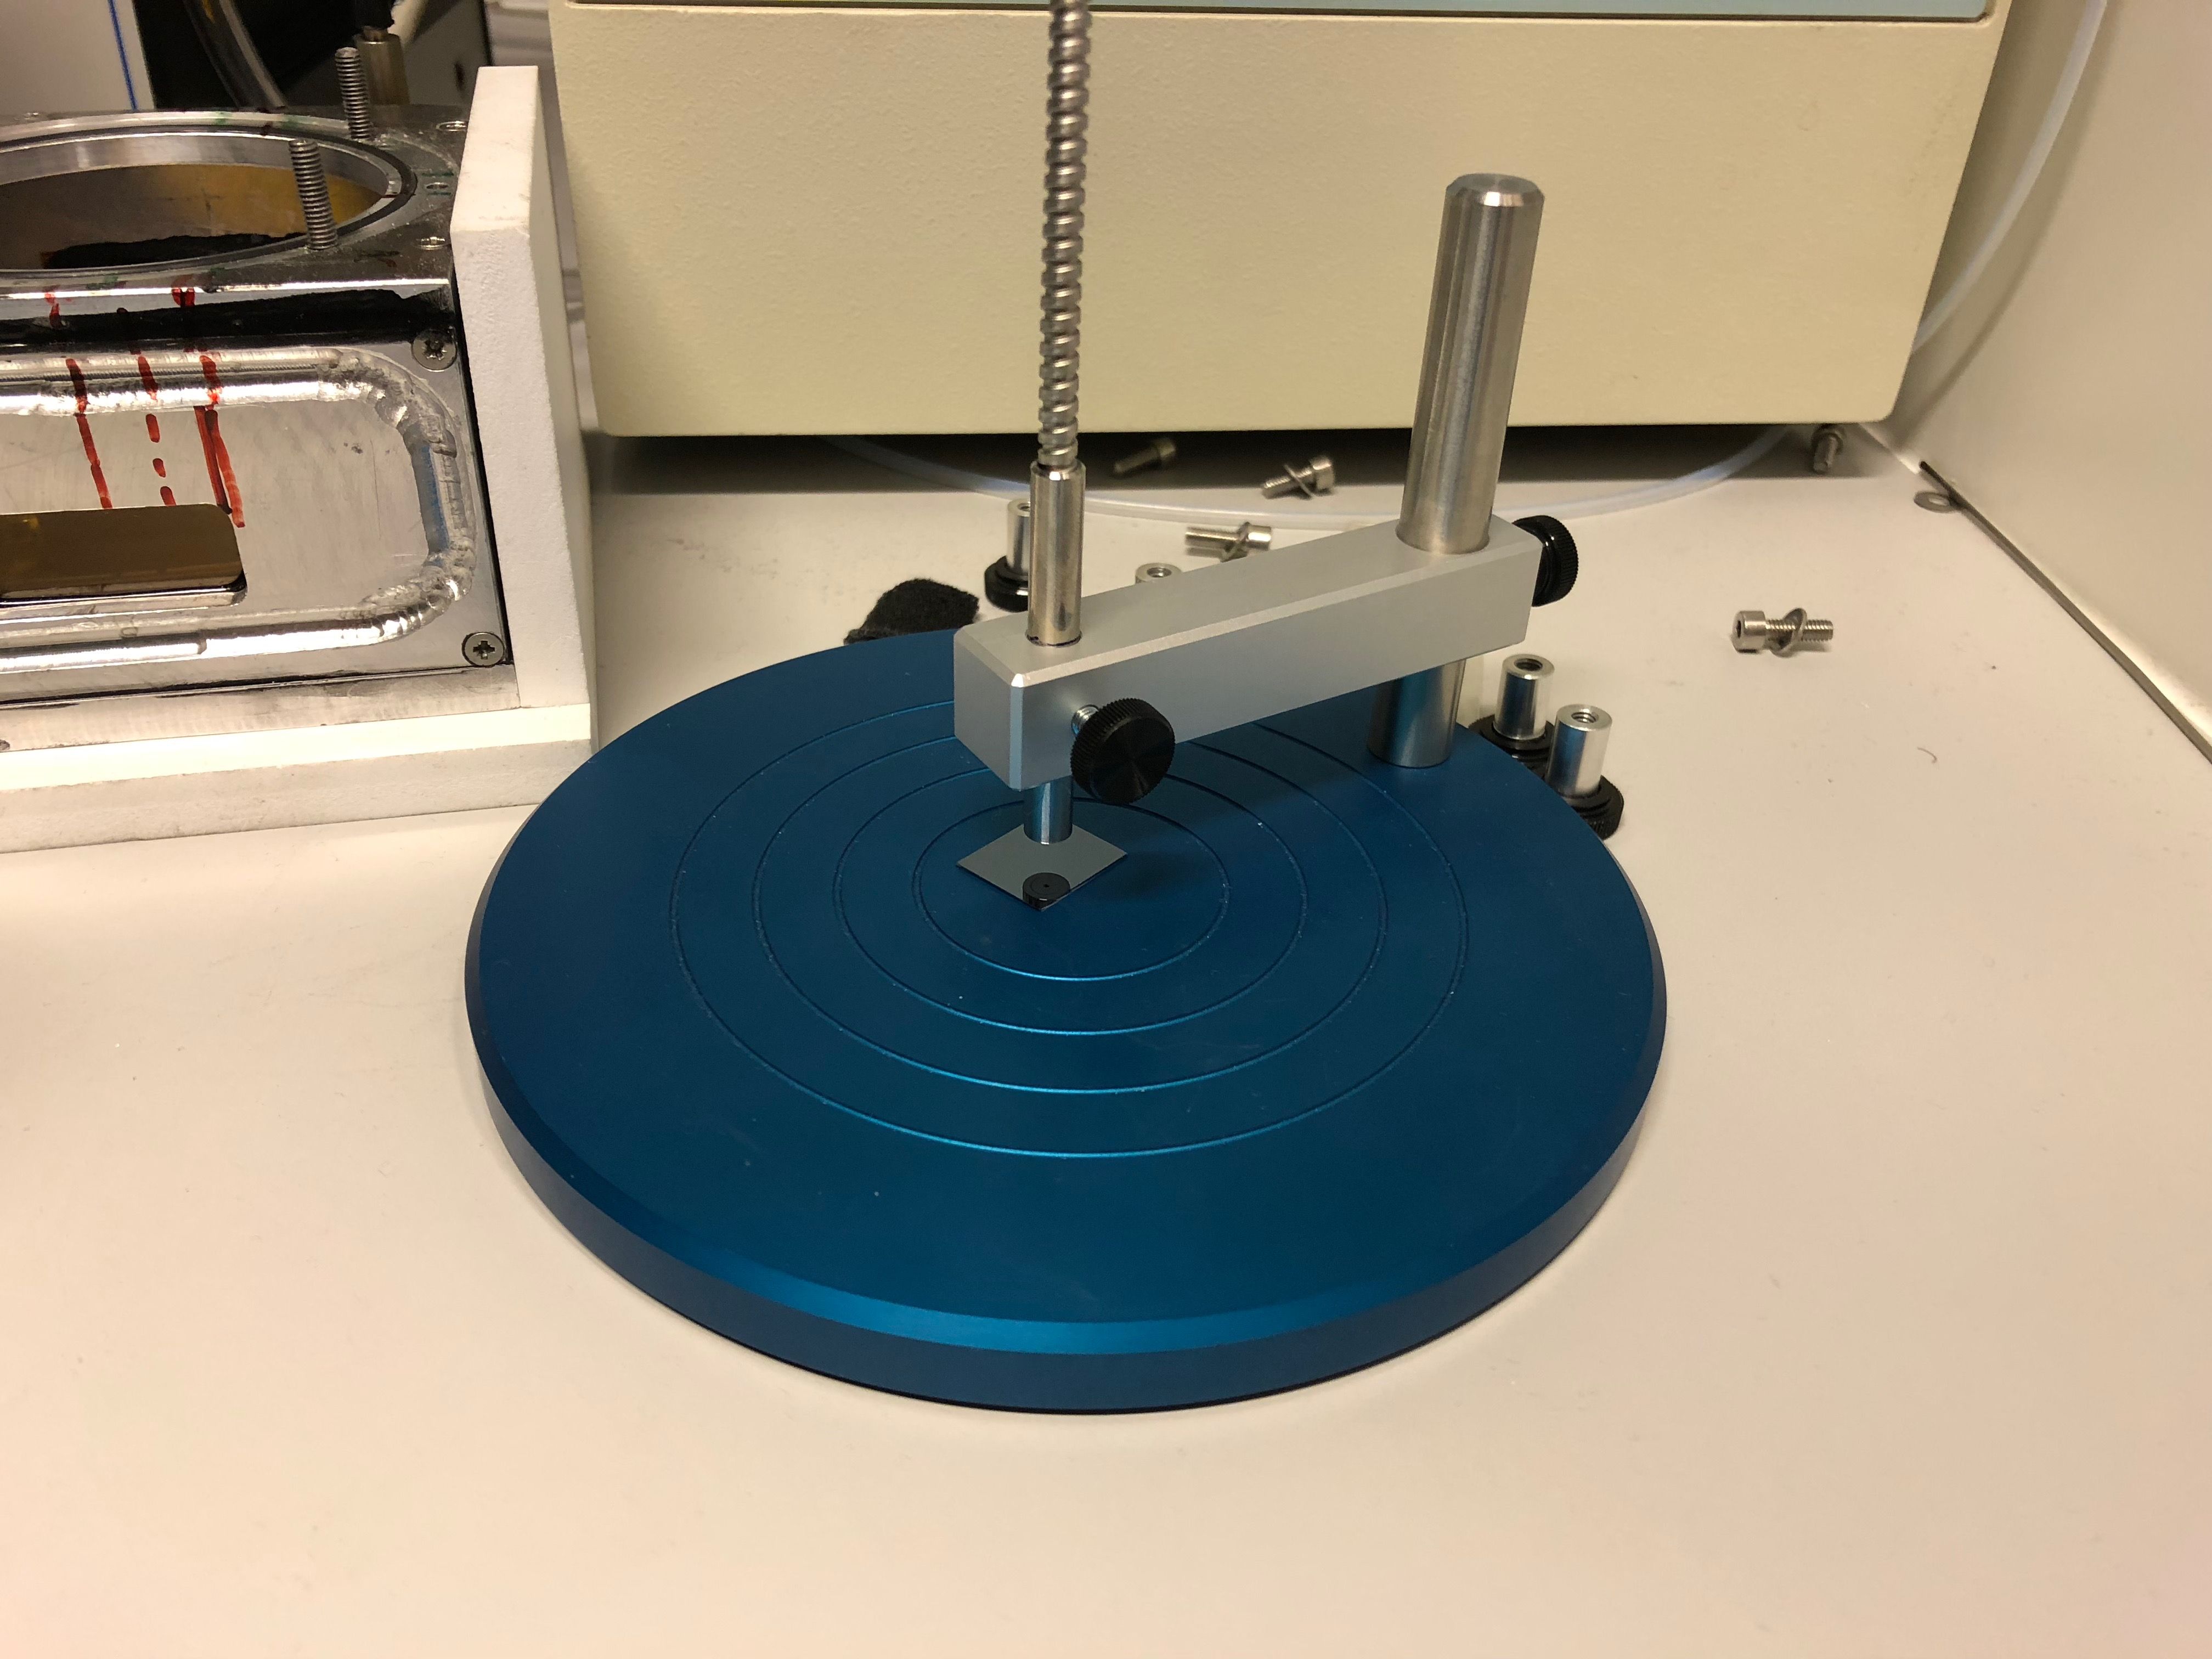
\includegraphics[width=.9\linewidth]{setup3.JPG} 
	    \caption{Single point stage} 
	    \label{fig:Singlestage}
	    \vspace{4ex}
	  \end{minipage}%% 
	  \begin{minipage}[b]{0.5\linewidth}
	    \centering
	    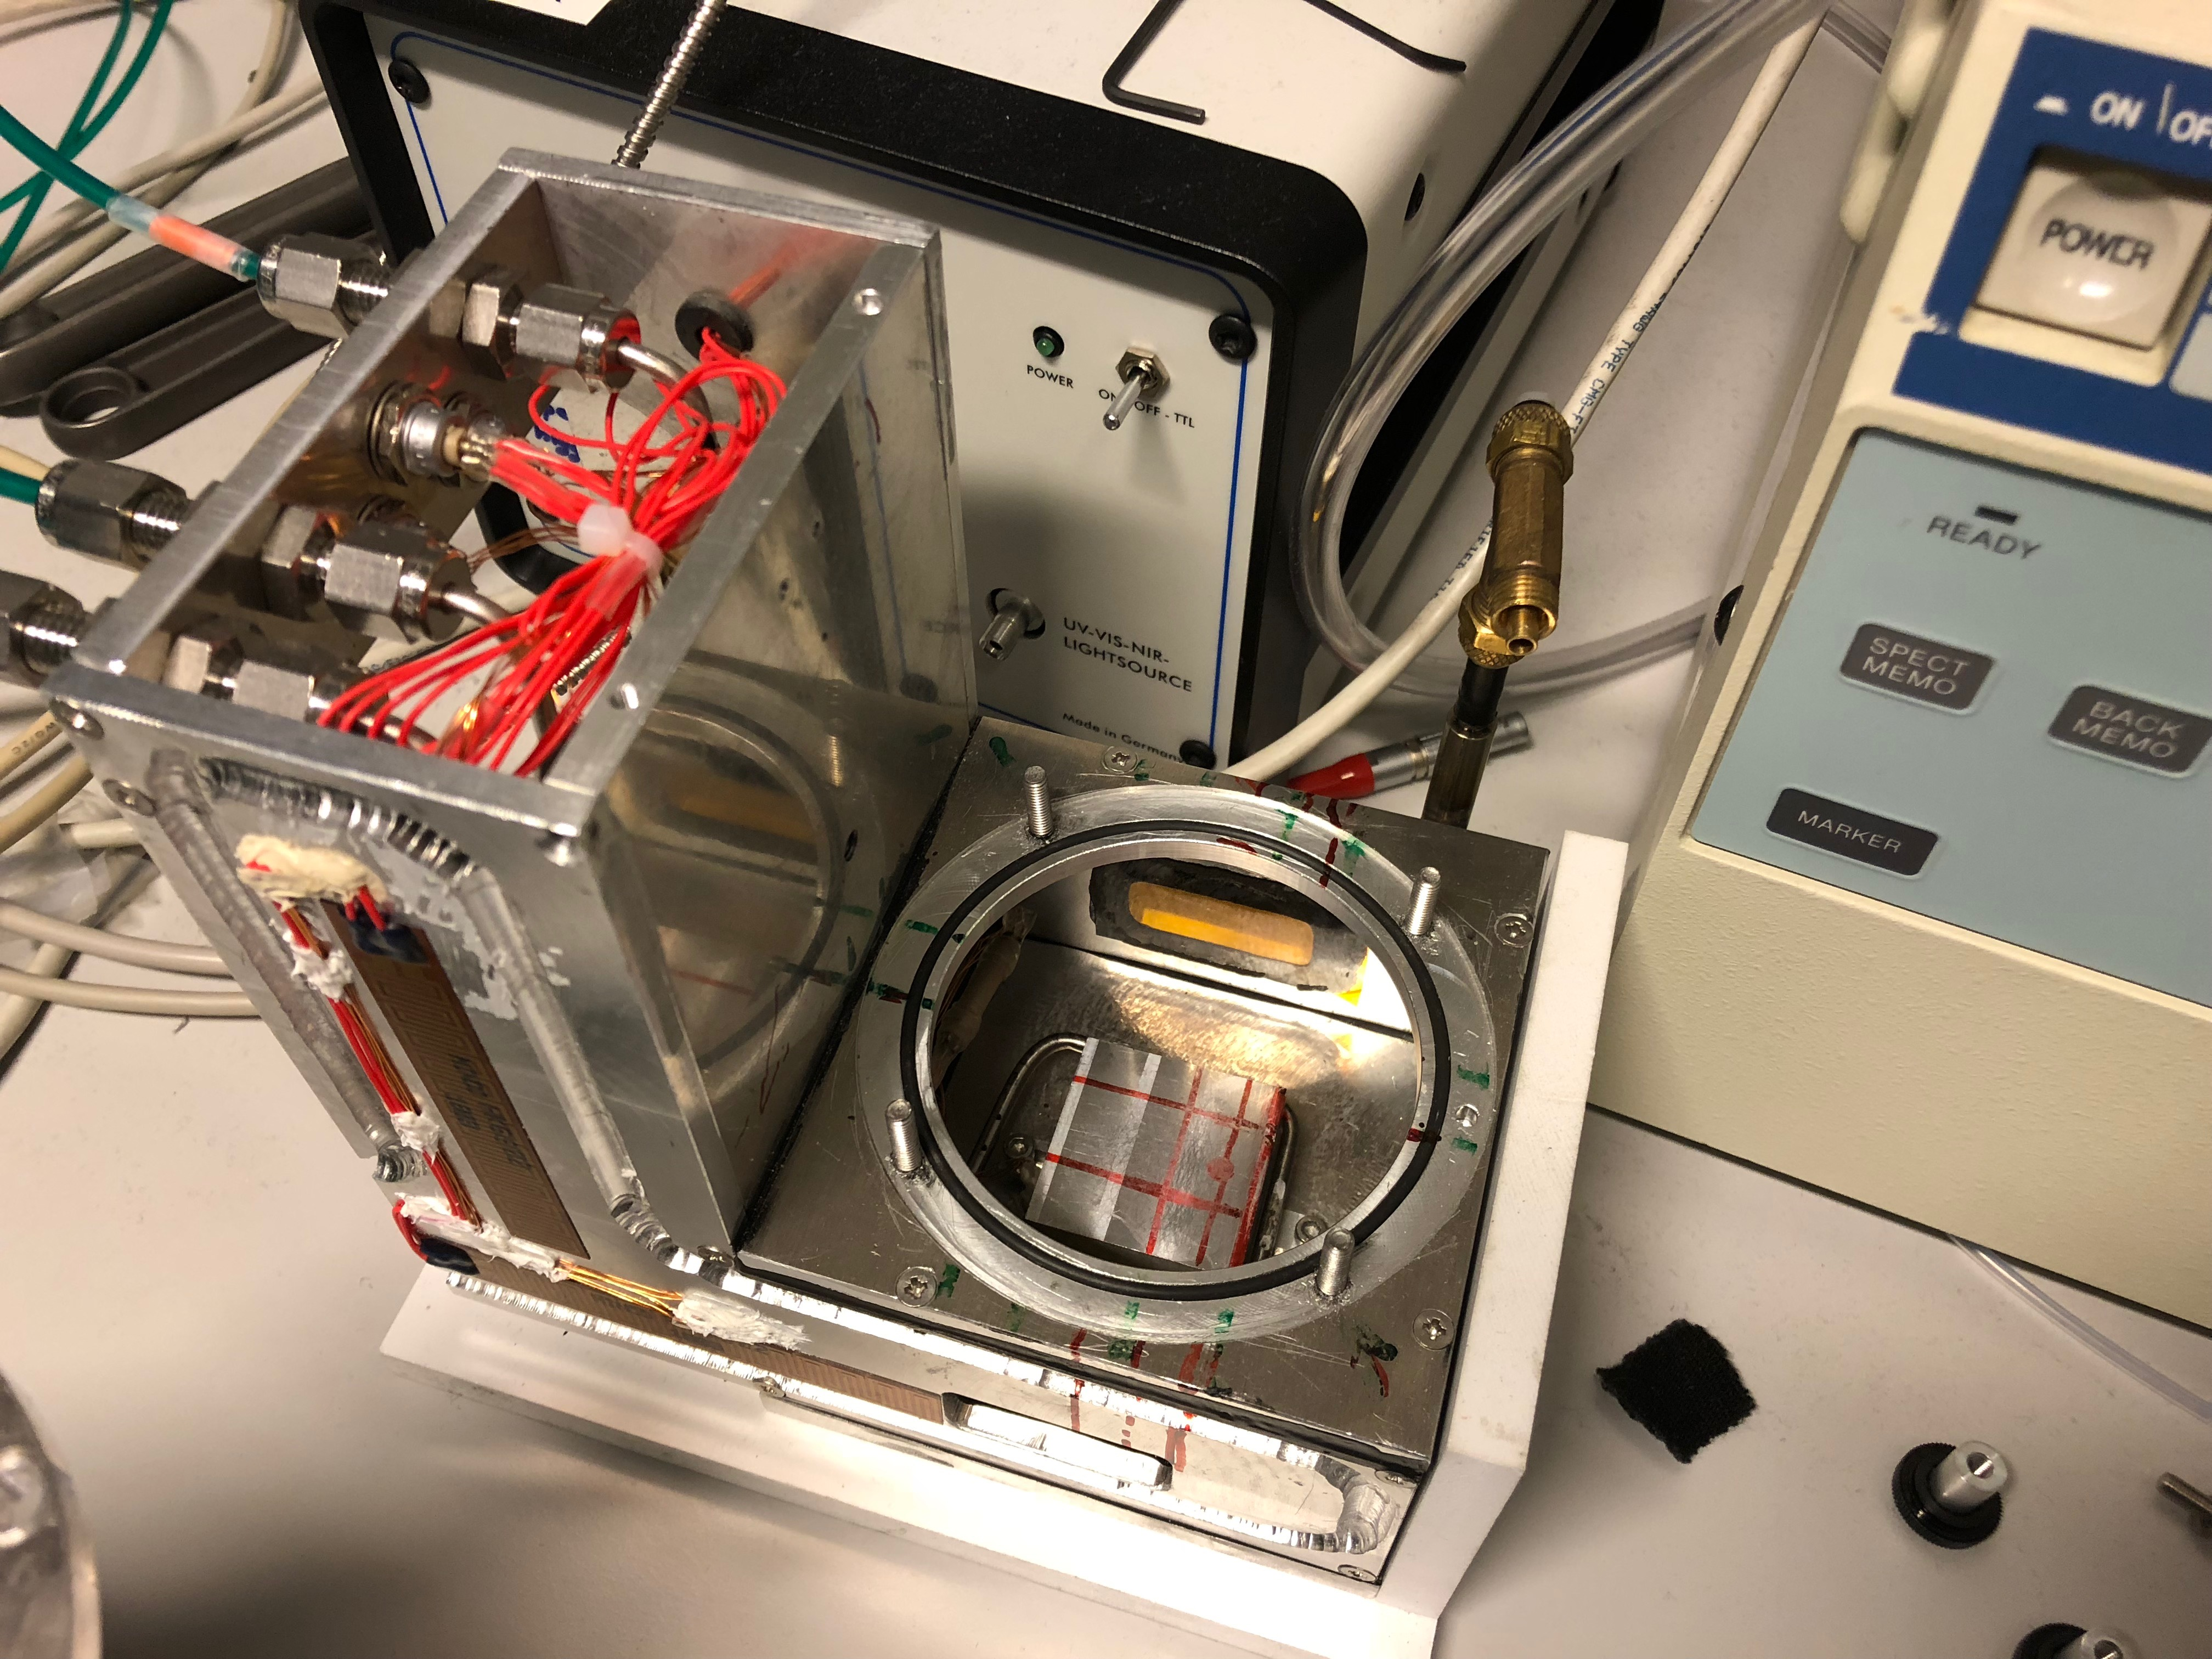
\includegraphics[width=.9\linewidth]{setup4.JPG} 
	    \caption{SVA experimental chamber \break minus lid}
	    \label{fig:SVAchamber} 
	    \vspace{4ex}
	  \end{minipage} 
	\end{figure}
	
	\begin{figure}
	\centering
		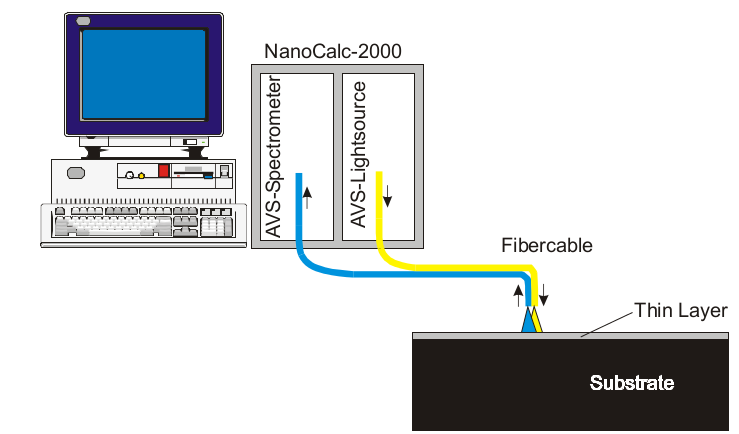
\includegraphics[width=\textwidth]{nanocalcsetup.png}
		\caption{This figure describes the NanoCalc set-up and has been taken from \cite{nanocalcmanual}. Light from a light source travels down the optical fiber illuminating the sample. The reflected light is collected by the optical fiber and analysed in the spectrometer. The spectrometer is connected to the computer by USB and the data is stored, modelled and manipulated through the NanoCalc software.}
		\label{fig:nanocalcsetup}
	\end{figure}
	
\section{Reflectance measurements in the NanoCalc spectrometer}
The NanoCalc spectrometer measures three light intensities which will be called a measurement onwards. The three measurements are the dark measurement (dark), the reference measurement (ref) and the thin-film measurement (meas). The dark measurement is the amount of light received by the optical fiber from external sources. The reference measurement is the amount of light reflected from a blank silicon wafer and the thin film measurement is the amount of light reflected from the sample. From chapter \ref{ch:reflect/trans}, the reflectance of a sample can be expressed as :

\begin{equation}\label{eq:nanocalcrefl}
R_{sample} = \frac{I_{sample}}{I_{incident}}.
\end{equation}

The spectrometer does not measure the intensity of the incident light, therefore the reflectance of the substrate is used to isolate the incident light intensity and inserted into equation \ref{eq:nanocalcrefl}. The reflectance of the substrate is used because it is easily calculated using the Fresnel equations as described in chapter \ref{ch:fresnelref}.

\begin{align}
R_{ref} = \frac{I_{ref}}{I_{incident}}\\
\implies  I_{incident} = \frac{I_{ref}}{R_{ref}} \label{eq:nanocalcrefl2}.
\end{align}

Inserting equation \ref{eq:nanocalcrefl2} in equation \ref{eq:nanocalcrefl}, the reflectance for the sample is expressed without the incident light intensity as:

\begin{equation}
R_{sample} = \frac{I_{sample}}{I_{ref}} \cdot R_{ref}.
\end{equation}

The reflectance of the sample is given as:

\begin{equation}
Reflectance = \frac{Meas-Dark}{Ref-Dark} \cdot R_{sub}.
\end{equation}

This is the same expression given in the NanoCalc spectrometer manual \cite{nanocalcmanual}. Through reproduction of the data and curves given by the NanoCalc spectrometer, i can deduce that the reference measurement has already had the dark measurement subtracted, giving the following reflectance expression:

\begin{equation}\label{eq:nanocalcreflect}
Reflectance = \frac{Meas-Dark}{Ref} \cdot R_{sub}.
\end{equation}

Placing equation \ref{eq:nanocalcreflect} equal to the reflectance equations using the Fresnel equations from chapters  \ref{ch:fresnelref}, \ref{ch:fresnel2lay} and \ref{ch:fresnelmulti}, the NanoCalc spectrometer software can fit a thickness of the sample.


\section{Reflectance measurement protocol}
In this section the experimental protocol for both taking measurements without the optics and with the optics are given. The halogen light source has been turned on 30 minutes prior to taking the measurements and the thin films have had 30 minutes to climatise to room temperature. The single point stage is set up and tested using a reference step wafer of known thicknesses. The protocol will be formulated in steps.

\subsection{Without Optics}
\begin{enumerate}
\item Take a continuous reference measurement and adjust the light intensity, such that the reference measurements maximum is $50\%$ of the y-axis.
\item Clear the reference measurement.
\item Take the optic fiber and point it away from anything that can reflect light. Take a dark measurement.
\item Place the optic fiber into ocean optics single point stage. The optic fiber is positioned $4$mm above the single point stage.
\item Place a blank silicon wafer under the optic fiber and take a reference measurement.
\item Save the dark and reference measurement.
\item Place a thin film under the optical fiber and take a measurement.  
\end{enumerate}

\subsection{With Optics}
\begin{enumerate}
\item Take a continuous dark measurement with the optic fiber with a dark cloth in the optics where the thin film would lie and adjust the light intensity, such that the dark measurements maximum is at 100$\%$ of the y-axis.
\item Clear the dark measurement.
\item Take the optics as a whole and point it away from anything that can reflect. Take a dark measurement.
\item Place a blank silicon wafer into the test chamber and place the optics into the test chamber. Take a reference measurement.
\item Save the dark and reference measurement.
\item Take the optics off the test chamber, remove the blank silicon wafer and place in a thin film sample. Place the optics onto the test chamber. Take a measurement.
\end{enumerate}

\section{Fitting of the reflectance data} \label{sec:fitting}
The mean square error is used when fitting the Fresnel equations to the reflectance measurements. The mean square error is given by:

\begin{equation}
MSE = \frac{1}{n}\sum_{i=1}^{n}\left( Y_i - \hat{Y}_i \right)^2,
\end{equation} 
where $n$ is equal to the amount of data points used, $Y_i$ is the measured value and $\hat{Y}_i$ is the estimated value. The fitting range is from $\SI{450}{\nano\meter}$ to $\SI{900}{\nano\meter}$. This range has been chosen ...[ARGUMENT HERE]. The parameters used in the fitting of Fresnel equations are the ambient refractive index $n_0$, the thin film refractive index $n_1$ and the thin film thickness $d_1$. The thickness for the silicon oxide layer is fixed at $\SI{2}{\nano\meter}$ and the complex refractive index values at each wavelength has been taken from Ocean Optics software. The complex refractive index for the silicon substrate has also be taken from the Ocean Optics software. Both the refractive indices for ambient and thin film are fitted for real numbers. The fitting scripts loops through the three parameter arrays calculating the mean square error for the measured reflectance data, finds the smallest mean square error value and saves the three parameters associated the smallest mean square error into an array. The next reflectance measurement is loaded in and the process begins again.

\section{Bronkhorst mass flow meters}
To regulate the solvent vapour annealing process, the experimental setup includes three Bronkhorst mass flow meters. This is important since controlling the vapour flow in different ways changes the structuring of the polymers when swelling. One EL-Flow select(F-201CV-500) with a flow capability for $N_2$ of  $\SI{4}{\milli\litre\per\minute}$ to $\SI{750}{\milli\litre\per\minute}$, or $400$ SCCM (Standard centimetre cubed per minute at $\SI{1}{\atmos}$ and $\SI{273}{\kelvin}$). Two EL-Flow select(F-201CV-200) with a $N_2$ flow of $\SI{1.6}{\milli\litre\per\minute}$ to $\SI{300}{\milli\litre\per\minute}$, or $200$ SCCM (Standard centimetre cubed per minute at $\SI{1}{\atmos}$ and $\SI{273}{\kelvin}$) \cite{elflow}.

During the both swelling processes, the SCCM will be kept constant to $200$ SCCM, with the assumption that the flowrate is constant through the system. When nitrogen flows through the bubbler and solvent the flowrate will change and thus the pressure in the SVA chamber will change. 


\section{Solvent Vapour Annealing Process}
The solvent vapour annealing process is divided into two process, a swelling and a drying process. In the swelling process a dry polymer upon a wafer is placed into the annealing chamber and is subjected to nitrogen gas. Slowly nitrogen gas is decreased and nitrogen gas through a bubbler filled with a solvent, in this thesis toluene, is increased creating vapour in the annealing chamber. When performing SVA, a solvent is chosen that is either neutral or slightly selective towards one of the polymers in the block copolymer. Solvent uptake is also dependant on the physical state of the block copolymer and the block fraction volume. The thin film will swell due to thermodynamic driving forces associated with the entropy of mixing of vapour and polymer blocks. The swelling will continue until the chemical potential of the vapour and the solvent in the thin film is in equilibrium. A diffusion front will arise continuing through the thin film from the vapour interface through to the substrate. It is published that the vapour pressure is an important thin film thickness parameter and should be controlled throughout the annealing. The vapour pressure is dependant on the mass flow controller, temperature of the solvent and temperature of the annealing chamber. The time taken to fully swell is also dependant on how organised the dry thin film is before swelling, this leads to varying swelling time. In a solvent swollen state the mobility of the polymer chains increase and the polymer can move in the volume of the thin film. The molar mass of the polymer plays at role in the how fast the polymer self assembles and a equilibrium state may not be achieved during the swelling. In the drying step the nitrogen gas flow through the bubbler is decrease and the direct nitrogen gas flow is increased. The solvent in the thin film is evaporated and the rate in which the solvent evaporates has been seen to have an impact of the nanoscale structure, in effect of quenching an organised structure. It is documented that both fast and slow evaporation leads to organised structure in block copolymers. An ordering front forms in the thin film during the evaporation where the thin film show order closer to the vapour interface and as the front propagates through the film, order follows in its wake\cite{SVABCP}. 

Structure characterisation is important during the stages of solvent vapour annealing, different experimental method illuminate different parameters. Spectral reflectometry used in this thesis will investigate how the thickness of the thin film evolves during SVA and shed light on how the refractive index for the ambient and thin film could evolve. 


\subsection{Solvent vapour annealing protocol} \label{sec:svaprotocol}
The solvent vapour annealing protocol used is a slow swell up to maximum toluene vapour flow which takes $\SI{5500}{\second}\approx\SI{92}{\minute}$ and a slow deswell which is the reverse of the slow swell up to the maximum taking $\SI{4000}{\second}\approx\SI{67}{\minute}$ to fully dry back roughly the thin films start thickness. The SVA takes a total of $\SI{158}{\minute}$ to run. The slow swell is broken up into five regions, the first region channel 1 dry nitrogen gass ($400$SCCM) is set to $50 \%$ for $\SI{1000}{\second}$. In the second region, channel 1 drops to $37.5 \%$ and channel 2 which flows through the bubbler increases from $0 \%$ to $25 \%$ for $\SI{1000}{\second}$. The third region, channel 1 drops to $25 \%$ and channel 2 increases to $50 \%$ for $\SI{1000}{\second}$. The fourth region, channel 1 drops to $12.5 \%$ and channel 2 increases to $75 \%$ for $\SI{1000}{\second}$. The fifth region, channel 1 drops to $0 \%$ and channel 2 increases to its maximum $100 \%$ for $\SI{1500}{\second}$. The solvent concentration can be calculated by the solvent loading of the thin film though the volume concentration, which can be expressed using the thickness. The solvent concentration is expressed as:

\begin{equation}
\phi= \frac{V_{solvent+film}-V_{film}}{V_{solvent+film}} = \frac{t_{solvent+film}-t_{film}}{t_{solvent+film}} = 1+\frac{t_{film}}{t_{solvent+film}}, 
\end{equation}
where $V$ is the volume of the thin film, and $t$ is the thickness of the thin film \cite{solventconcentration}.

During the solvent vapour annealing protocol a reflectance measurement is taken every $10$ seconds and saved into its own .dat file. The solvent vapour annealing protocol is controlled by a script loading into the Bronkhorst Flowplot software.The script is called slowslow.fps and has been included in the appendix \ref{app:slowslow} of this thesis.

\begin{figure}
\centering
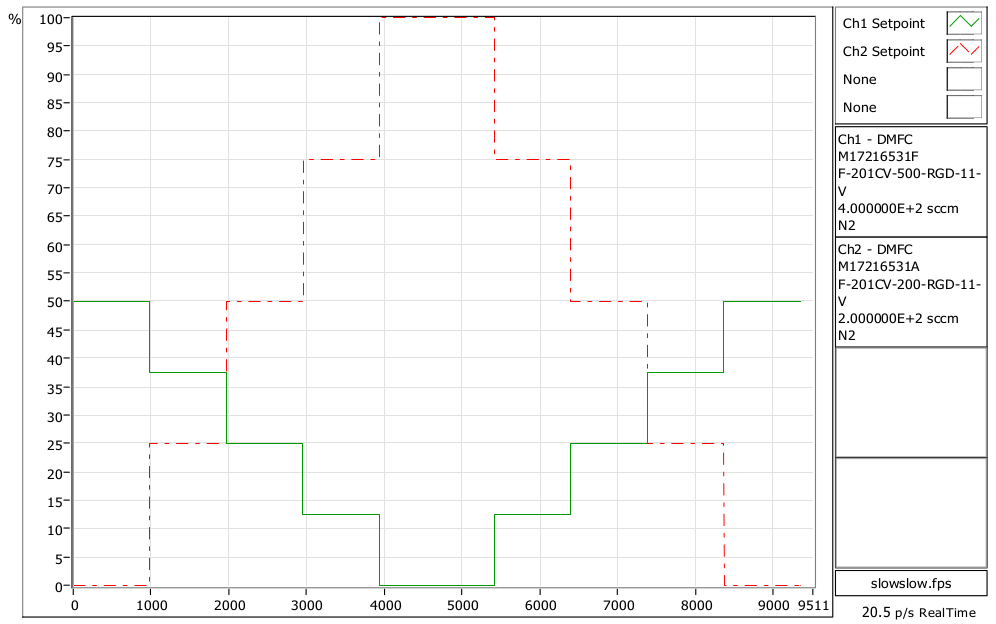
\includegraphics[width=\textwidth]{slowslowprotocol.png}
\caption{Slow swelling and slow deswelling protocol. Along the x-axis, time is shown in seconds, the full SVA protocol taking $\SI{9500}{\second}$. Along the y-axis, how hard the mass flow meter is working in procent. The green plot belongs to the $400$SCCM Bronkhorst mass flow meter controlling the nitrogen gas and the red dashed plot belongs to the $200$SCCM Bronkhorst mass flow meter controlling the nitrogen flowing through the bubbler. The swelling is done by loading a swelling script called slowslow.fps show in appendix \ref{app:slowslow}.}
\label{fig:slowslow}
\end{figure}
   



\end{document}